\documentclass[border=10pt]{standalone}
\usepackage[svgnames]{xcolor}
\usepackage{amsmath}
\usepackage{pgfplots}
\pgfplotsset{compat=newest}
\usepackage[sfdefault]{FiraSans}
\usepackage{FiraMono}
\renewcommand*\familydefault{\sfdefault}
\begin{document}
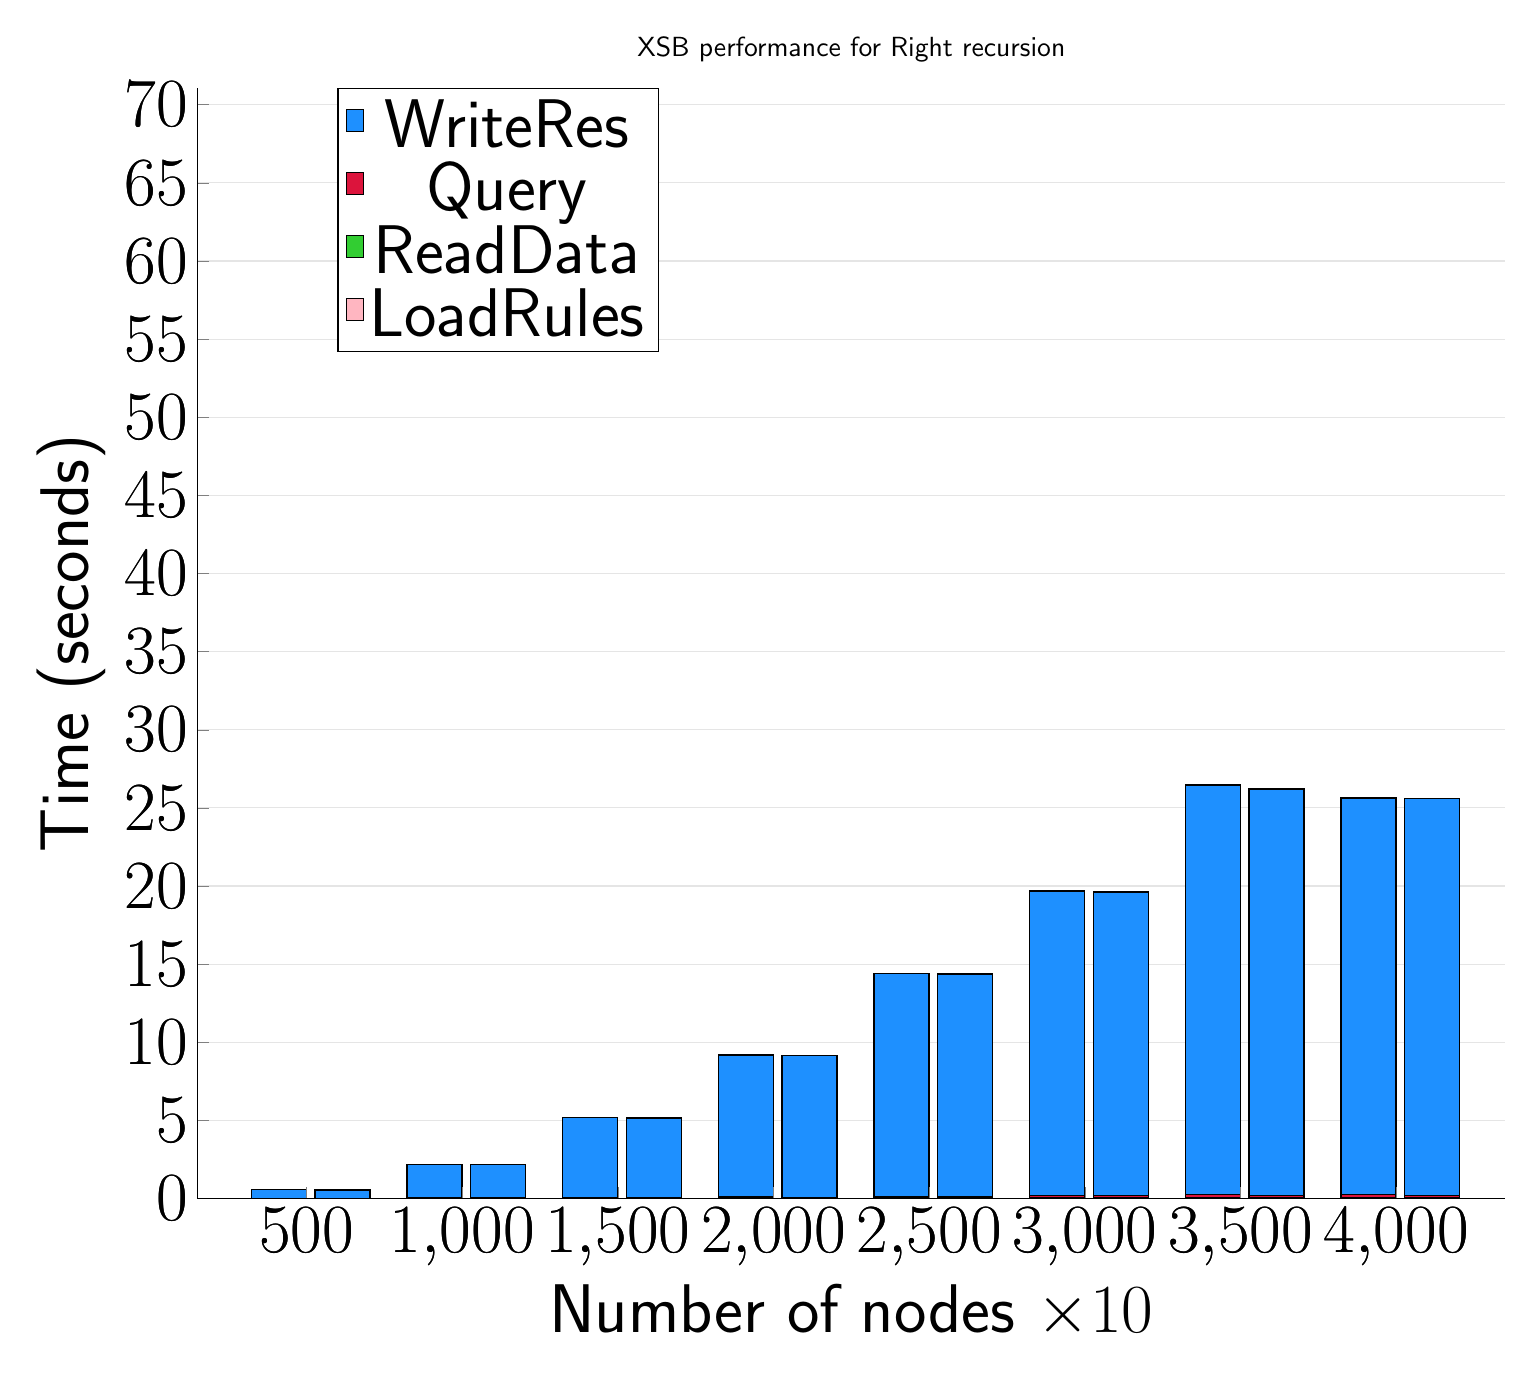
\begin{tikzpicture}
\begin{axis}[
   ybar stacked,
   title={XSB performance for Right recursion},
   bar shift=-10pt,
   width=1.5\textwidth,
   bar width=0.7cm,
   ymajorgrids, tick align=inside,
   major grid style={draw=gray!20},
   xtick=data,
   ymin=0, ymax=71.079008658727,
   axis x line*=bottom,
   axis y line*=left,
   enlarge x limits=0.1,
   legend style={
       at={(0.23, 1)},
       anchor=north,
       legend columns=1,
       font=\Huge,
   },
   ylabel={Time (seconds)},
   xlabel={Number of nodes $\times 10$},
   label style={font=\Huge},
   tick label style={font=\Huge},
]
\addlegendimage{fill=DodgerBlue, draw=black, line width=0.2pt}
\addlegendentry{WriteRes}
\addlegendimage{fill=Crimson, draw=black, line width=0.2pt}
\addlegendentry{Query}
\addlegendimage{fill=LimeGreen, draw=black, line width=0.2pt}
\addlegendentry{ReadData}
\addlegendimage{fill=LightPink, draw=black, line width=0.2pt}
\addlegendentry{LoadRules}
\addplot +[fill=LightPink, draw=black, line width=0.5pt] coordinates {
    (500, 0.0059163570404052734)
    (1000, 0.004241943359375)
    (1500, 0.004408359527587893)
    (2000, 0.0046727657318115234)
    (2500, 0.004613002141316731)
    (3000, 0.004548311233520507)
    (3500, 0.004677931467692056)
    (4000, 0.0038415590922037768)
};
\addplot +[fill=LimeGreen, draw=black, line width=0.5pt] coordinates {
    (500, 0.010203282038370766)
    (1000, 0.014702002207438133)
    (1500, 0.021538019180297834)
    (2000, 0.027882973353068035)
    (2500, 0.0376269817352295)
    (3000, 0.04695741335550943)
    (3500, 0.04959535598754883)
    (4000, 0.0478196938832601)
};
\addplot +[fill=Crimson, draw=black, line width=0.5pt] coordinates {
    (500, 0.006180763244628907)
    (1000, 0.015395959218343067)
    (1500, 0.03493197758992513)
    (2000, 0.062095324198404966)
    (2500, 0.09647901852925611)
    (3000, 0.15647292137145966)
    (3500, 0.20122869809468602)
    (4000, 0.19631004333496102)
};
\addplot +[fill=DodgerBlue, draw=black, line width=0.5pt] coordinates {
    (500, 0.5395468870798744)
    (1000, 2.1627410252889003)
    (1500, 5.115908702214559)
    (2000, 9.100783348083509)
    (2500, 14.273369232813543)
    (3000, 19.46644735336304)
    (3500, 26.201669216156017)
    (4000, 25.375265041987074)
};
\end{axis}
\begin{axis}[
   ybar stacked,
   bar shift=13pt,
   width=1.5\textwidth,
   bar width=0.7cm,
   ymajorgrids, tick align=inside,
   major grid style={draw=none},
   xtick=data,
   ymin=0, ymax=71.079008658727,
   axis x line*=none,
   axis y line*=none,
   enlarge x limits=0.1,
   label style={font=\Huge},
   tick label style={font=\Huge},
]
\addplot +[fill=LightPink, draw=black, line width=0.5pt] coordinates {
    (500, 0.00547)
    (1000, 0.004241000000000003)
    (1500, 0.0033830000000000006)
    (2000, 0.0018150000000000013)
    (2500, 0.004612000000000001)
    (3000, 0.002747333333333333)
    (3500, 0.003839)
    (4000, 0.003145666666666667)
};
\addplot +[fill=LimeGreen, draw=black, line width=0.5pt] coordinates {
    (500, 0.010071666666666666)
    (1000, 0.014701333333333335)
    (1500, 0.021458666666666668)
    (2000, 0.023836333333333334)
    (2500, 0.03762133333333333)
    (3000, 0.04518266666666667)
    (3500, 0.049007)
    (4000, 0.04779066666666667)
};
\addplot +[fill=Crimson, draw=black, line width=0.5pt] coordinates {
    (500, 0.0061226666666666625)
    (1000, 0.015392333333333333)
    (1500, 0.032133)
    (2000, 0.0522)
    (2500, 0.090911)
    (3000, 0.132877)
    (3500, 0.16262466666666667)
    (4000, 0.15316466666666667)
};
\addplot +[fill=DodgerBlue, draw=black, line width=0.5pt] coordinates {
    (500, 0.5363096666666666)
    (1000, 2.1558703333333336)
    (1500, 5.097248666666666)
    (2000, 9.083624333333335)
    (2500, 14.248230999999999)
    (3000, 19.436594333333332)
    (3500, 25.986491666666666)
    (4000, 25.386606999999998)
};
\end{axis}
\end{tikzpicture}

\end{document}
